% ============================================================================
% DHG508 Final Design Paper & Post-Mortem
% 北宋赶考记 · 嘉祐二年 (A Scholar's Road to Bianjing, 1057)
% Lingnan University — Critical Digital History
%
% OVERLEAF SETUP:
%   1. Upload this paper/ folder (zipped) to Overleaf (New Project -> Upload Project)
%   2. Menu (top left) -> Compiler -> XeLaTeX
%   3. Click Recompile (Biber + Noto Serif CJK SC run automatically)
% ============================================================================

\documentclass[12pt,a4paper]{article}

\usepackage{fontspec}
\newcommand{\MainLatinFont}{Times New Roman}
\newcommand{\FallbackLatinFont}{TeX Gyre Termes}
\newcommand{\MainCJKFont}{Noto Serif CJK SC}
\newcommand{\FallbackCJKFont}{FandolSong-Regular.otf}

\IfFontExistsTF{\MainLatinFont}
  {\setmainfont{\MainLatinFont}}
  {\setmainfont{\FallbackLatinFont}}

\usepackage{xeCJK}
\IfFontExistsTF{\MainCJKFont}
  {\setCJKmainfont{\MainCJKFont}}
  {\IfFontExistsTF{Songti SC}
    {\setCJKmainfont{Songti SC}}
    {\IfFontExistsTF{SimSun}
      {\setCJKmainfont{SimSun}}
      {\setCJKmainfont{\FallbackCJKFont}}}}

\usepackage[a4paper, margin=1in]{geometry}
\usepackage{setspace}
\usepackage{booktabs}
\usepackage{array}
\usepackage{graphicx}
\usepackage{csquotes}

% Chicago Manual of Style 18th ed., Notes-Bibliography (BibLaTeX + Biber)
\usepackage[notes, backend=biber, autolang=other, isbn=false]{biblatex-chicago}
\addbibresource{references.bib}

\renewcommand{\footnotesize}{\fontsize{10}{12}\selectfont}
\usepackage[hidelinks]{hyperref}

\title{\textbf{North Song Examination Run: A Historical Simulation of the \emph{Jiayou} 2 (1057) Metropolitan Examination}\\[0.3em]
\large Design Rationale, Evidence Boundaries, and Post-Mortem}
\author{Zhang Min\\Lingnan University $\cdot$ DHG508 Critical Digital History\\
\small Live URL: \url{https://songgame.pages.dev} $\cdot$ Repo: \url{https://github.com/echozhangmin/songgame}}
\date{25 November 2026}

\begin{document}
\maketitle

\begin{abstract}
\noindent
This paper documents the design, evidence boundaries, and verification of
\emph{North Song Examination Run} (\emph{Bei Song Gan Kao Ji}), a single-file
HTML simulation of the 1057 metropolitan examination cycle. The player is a
degree-holder from Linchuan who travels thirty days to Bianjing and passes
through the documentary, financial, and epistemic machinery of the Song
examination system: certification, registration, the three anonymised
examination sessions, and the palace ranking. Every one of the game's 57
glossary claims is tagged as \emph{ju} (documented), \emph{tui} (inferred), or
\emph{she} (invented), with a hard epistemic cutoff at 1057. Four layers of
automated tests (540 full simulation runs, a 54-case interactive walkthrough,
poem-grading and dialogue suites) and two external playtests, each converted
into regression tests, hold the build together. The paper argues that a
simulation teaches what film cannot: examination success as \emph{management},
not merely talent.
\end{abstract}

\onehalfspacing

\section{Historical Question and Medium}

The \emph{Jiayou} 2 (1057) examination cohort is remembered as the most
illustrious in Chinese history: Su Shi, Su Zhe, Zeng Gong, Cheng Hao, Zhang
Zai, and L\"{u} Huiqing passed in the same year under examiner Ouyang Xiu.
That lustre, however, is hindsight. For an ordinary candidate without a
biography, 1057 was first of all a machine: an autumn prefectural
qualification (\emph{jie} examination), a thousand-mile journey with limited
funds, the ritual of registration at the Ministry of Rites, three examination
sessions graded blind under cover-name and transcription rules, and the
final ranking. This project asks: \textbf{what did that machine feel like to
pass through, and why did most candidates fail?}

A static essay or documentary can only describe that passage; a simulation
makes a reader \emph{be} the candidate. Three mechanics carry the argument.
First, \emph{trade-offs}: each in-game day grants four action points, and
studying, resting, socialising, and spending compete for them; on travel
days only two remain, so something is always dropped. Second, an
\emph{embodied sense of institutions}: because cover-naming and transcription
were already in force,\autocite[juan 155]{songshi} the game's ``ask around
about the examiners'' action can only ever return rumour---anonymity shapes
candidate behaviour as a rule the player collides with, not a footnote. Third,
\emph{failure is systemic}: four independent death-lines (learning, health,
social capital, money) end the run; across 540 simulated runs, mid-ability
agents cluster in the lower degree tiers. Failing is not stupidity but
management failure---and unlike film, the player can replay and try a
different strategy.

\section{Sources and Scholarly Conversation}

\textbf{Primary sources.} The institutional skeleton is drawn from the
\emph{Song History: Treatise on Selection} (\emph{Song shi}, \emph{Xuanju
zhi} 1), in which the sequence ``poetry and rhapsody first, \emph{lun} essay
second, policy third'' and the calendar ``prefectural exams in autumn,
assemble at the Ministry in winter, examine in spring'' were verified against
the received text.\autocite[juan 155]{songshi} The lock-in of the examiners is
documented in Ouyang Xiu's \emph{Guitian lu}: in 1057 he and Han Jiang served
as chief examiners, recruited Mei Yaochen as checking official, and remained
sealed in the compound for fifty days, composing poetry together.\autocite{guitianlu}
The \emph{xing juan} (advance submission) custom is cited from Zhao Yanwei's
\emph{Yunlu manchao}.\autocite[juan 8]{yunlu} Kaifeng geography follows the
\emph{Dongjing meng hua lu}.\autocite{dongjingmenghualu} The limits are
declared: citations are at \emph{juan}/chapter level pending page-by-page
verification against the Zhonghua shuju punctuated editions; the detailed
itinerary from Linchuan to Bianjing is not attested in a single source and is
handled as a declared compression.

\textbf{Scholarly conversation.} Three works shape the design. Rong
Hengying's study of the 1057 triangle---chief examiner Ouyang Xiu, checking
official Mei Yaochen, and newly-minted \emph{jinshi} Su Shi---shows how
poetic exchange and letters of thanks generated ``elective affinity'' within
a strictly hierarchical institution; the game's master-scholar
\emph{conversations} (one topic per visit, with follow-up questions) are
built directly on this account.\autocite[175--193]{rong2019} John Chaffee's
social history of the Song examinations supplies the ``machine'' framing
itself---the three-tier system, quotas, and the social meaning of
failure---which the game's twelve scenes translate into levels of a
course.\autocite{chaffee1985} Miyazaki Ichisada's classic account of
examination life justifies the game's exhaustion, expense, and risk
mechanics, and its depiction of the examination compound as an ordeal rather
than a venue.\autocite{24--38}{miyazaki1976} The design responds to these
works at specific points listed in the evidence table (Section~4).

\section{Architecture and Boundaries}

The system is four layers. \textbf{Data}: \texttt{data/glossary.json}
(57 claims, each with a definition, source, note, and evidence-tier tag) and
\texttt{data/quiz\_150.json} (150 questions). \textbf{Logic}: a day-loop
state machine (four statistics, nightly settlement, four failure lines), a
poem grader, and event/dialogue systems, written without DOM dependencies so
that macOS's built-in JavaScript for Automation can execute them headlessly.
\textbf{Rendering}: a single-file HTML build (\texttt{build.py} inlines the
quiz, glossary, and twelve scene illustrations as base64). \textbf{Deployment}:
a split variant (\texttt{build.py -{}-dist}) converts illustrations to linked
WebP, shrinking the HTML from 7.9\,MB to 158\,KB, served on Cloudflare Pages
with one-year immutable caching; the single-file build is kept as the offline
edition. Figure~\ref{fig:schematic} shows the pipeline.

Epistemic boundaries are enforced, not merely declared. A pytest gate rejects
any glossary entry lacking a valid \emph{ju}/\emph{tui}/\emph{she} tag; quiz
items later than 1057 must carry an explicit \texttt{afterCutoff} flag; and
characters may not know what they could not have known (Huang Tingjian, aged
twelve in 1057, and Mi Fu, aged six, are deliberately absent).

\begin{figure}[htbp]
  \centering
  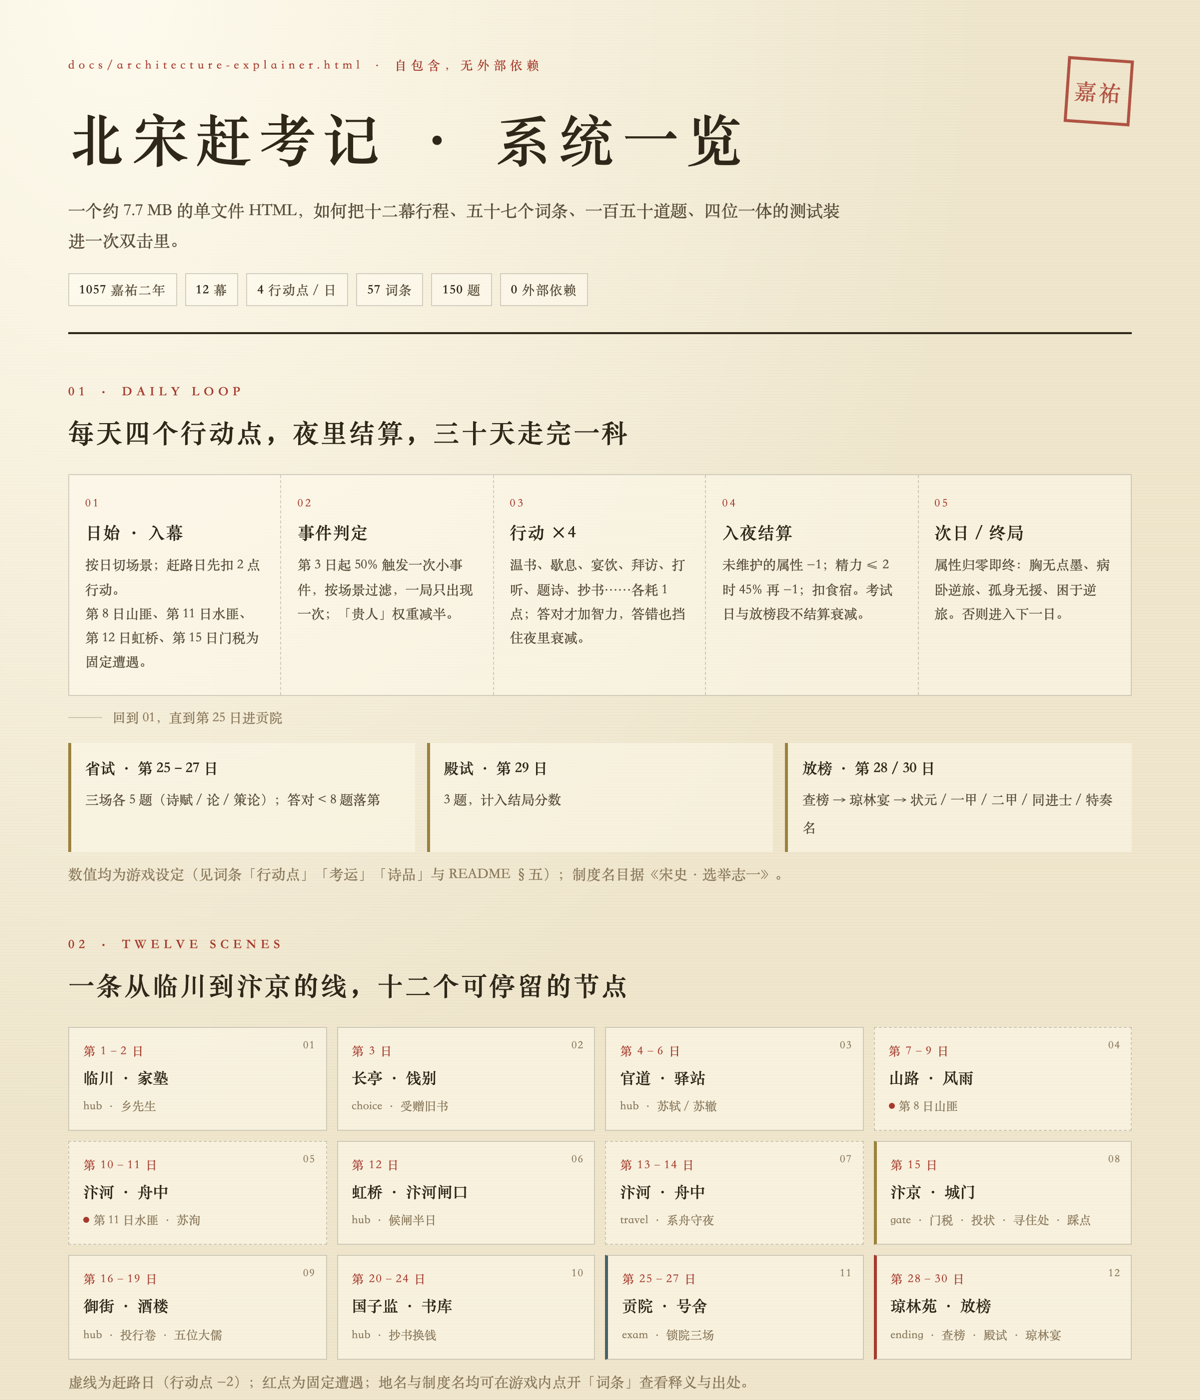
\includegraphics[width=0.92\textwidth]{schematic.png}
  \caption{Project architecture and interaction flow (agent-generated
  schematic, \texttt{docs/architecture-explainer.html}).}
  \label{fig:schematic}
\end{figure}

\section{Evidence Table}

All 57 glossary claims are exported to \texttt{evidence.csv} and compiled
into Table~\ref{tab:evidence} by \texttt{make\_evidence\_table.py}; no table
row is typed by hand. The tier distribution---\emph{ju} 5, \emph{tui} 49,
\emph{she} 3---is itself a methodological statement: the skeleton of a
playable 1057 is documented, the flesh is responsible inference, and pure
invention is small and explicitly labelled.

\begin{table}[htbp]
  \centering
  \footnotesize
  \singlespacing
  \renewcommand{\arraystretch}{1.25}
  % Auto-generated from evidence.csv by make_evidence_table.py — edit the CSV, not this file.
\begin{tabular}{p{0.27\textwidth}p{0.20\textwidth}p{0.13\textwidth}p{0.08\textwidth}p{0.22\textwidth}}
  \toprule
  \textbf{Claim / Element} & \textbf{Source / File} & \textbf{Locator} & \textbf{Level} & \textbf{Boundary / Limit} \\
  \midrule
  州府发给解试合格举人的文书。入京应省试时要验看，相当于准考证。 & 《宋史·选举志一》；《宋会要辑稿·选举》 & 州府解试中选者给解牒，许赴省试。；诸州解送举人，须具解状、家状投礼部，故宋人公文“解牒”“解状”并用。 & 推断 & 本作统一用“解状”。 \\
  州府主持的选拔考试，中式者称举人，才有资格赴京应省试。 & 《宋史·选举志一》 & 解试由州府长官主持，中选者贡于礼部。 & 推断 & — \\
  尚书省礼部主持的全国性考试，举人赴京应之，中式者再赴殿试。 & 《宋史·选举志一》 & 礼部贡院掌受诸州解送举人名籍，按期试之。 & 推断 & 本作第 25–27 日的三场即省试。 \\
  皇帝亲自主持的复试。宋初殿试有黜落，后渐成定例，主要定等第。 & 《宋史·选举志一》 & 省试中选者，天子亲策于廷，谓之殿试。 & 推断 & — \\
  省试的主考官，多由翰林学士、中书舍人等临时差充。 & 《宋史·选举志一》 & 以他官权知贡举，掌贡举之事。 & 推断 & 嘉祐二年知贡举为欧阳修，点检试卷官为梅尧臣。 \\
  考官受命后即入贡院锁宿，不许外出见客，以防请托泄题。 & 《宋史·选举志一》；欧阳修《归田录》 & 试官入贡院锁宿，不得与外人通。；欧阳修记嘉祐二年与韩绛同知贡举、辟梅尧臣为小试官，锁院五十日，唱和成集。 & 推断 & 锁院期间所作唱和诗，即《礼部唱和诗》。 \\
  把平日所作诗文投献给名公权要，求其延誉、向主司推荐。唐以来举子多行此风，宋初虽禁公荐，投卷仍不绝。 & 赵彦卫《云麓漫钞》卷八 & 唐之举人，先藉当世显人，以姓名达之主司，然后以所业投献；逾数日又投，谓之温卷。 & 据 & 本作把它做成一个动作：花 2 贯、耗 1 点行动，谒见知贡举欧阳修，智力与人缘各 +1，并留下“行卷”的考运；到京后会收到短笺。“考运加成”为游戏化设定——糊名誊录、公卷已罢之下， \\
  投卷之后再投一次，以加深印象。 & 赵彦卫《云麓漫钞》卷八 & 逾数日又投，谓之温卷。 & 据 & 本作未单独做“温卷”动作，投行卷一次即算完成。 \\
  科举中录取自己的考官。唐代门生称考官为“座主”、自称“门生”，宋初严禁此称，以防结党。 & 《宋史·选举志一》 & 宋初禁举子称考官为座主、自称门生，犯者抵罪。 & 推断 & 所以本作里举子只称“主司”，不称座主。 \\
  放榜后皇帝临轩，按名次逐一唱名，谓之唱名。 & 《宋史·选举志一》 & 赐第之日，天子临轩唱名，卫士传呼。 & 推断 & — \\
  举子把平日所作诗文投献给名公权要，求其延誉、向主司推荐。 & 赵彦卫《云麓漫钞》卷八 & 唐之举人，先藉当世显人，以姓名达之主司，然后以所业投献；逾数日又投，谓之温卷。 & 据 & 此为唐制记载。宋代作为贡举程序的“公卷”，在封弥誊录法行后已罢（《宋史·选举志一》：贾昌朝言“今有封弥、誊录法，一切考诸试篇，则公卷可罢”，“自是不复有公卷”）；作为社交干谒的投献 \\
  贡院内分隔的考生小屋，一人一间，答卷、食宿皆在其中。 & 《宋史·选举志一》 & 贡院分列廊庑，设席舍以居举人。 & 推断 & 宋人多称“席舍”“试廊”，“号舍”是后世通称。 \\
  糊去试卷上的姓名、乡贯，使考官不知作者，以防徇私。 & 《宋史·选举志一》 & 太宗淳化三年，殿试始行糊名考校。 & 推断 & — \\
  另设书吏将试卷誊抄一遍，考官只看抄本，以防辨认笔迹。 & 《宋史·选举志一》 & 真宗大中祥符八年，置誊录院，募书吏誊写试卷。 & 推断 & — \\
  屡试不第、年岁已高的举子，由礼部另列名奏上，附试后赐出身。 & 《宋史·选举志一》 & 士贡于乡而屡绌于礼部者，积其举数与年岁，别籍其名以奏，许附试，谓之特奏名。 & 推断 & 史实中特奏名须“积其举数与年岁”（屡试不第、年高者方得）；本作取作最低及第档的游戏性保底，结局页有自注。 \\
  及第等第之一，在“进士出身”之下，仍属正榜。 & 《宋史·选举志一》 & 及第分等：及第、进士出身、同进士出身。 & 推断 & — \\
  放榜后赐新科进士的宴席，设在琼林苑，故称。 & 《宋史·选举志一》 & 赐新及第进士宴于琼林苑，谓之琼林宴。 & 推断 & — \\
  赠给远行者的路费、盘缠。长亭饯别时亲友所赠即此类。 & 宋人书札 & 宋人多称“资装”“程费”，欧阳修、苏轼尺牍中屡见“资装”之语。 & 推断 & “程仪”多见于明清小说，宋代并非常语；本作用它作通称，取其易解。 \\
  路费、旅费。宋元以来口语，话本、元曲中常见。 & 宋元话本与元曲 & “盘缠”指旅途用度，屡见。 & 推断 & 本作把盘缠抽象为唯一货币；宋人实用铜钱、交子、金银，另有“驿券”可免费住驿。 \\
  城外十里一长亭、五里一短亭，是送别饯行之处。 & 李白《菩萨蛮》 & 何处是归程，长亭更短亭。 & 据 & 词中“长亭”已作送别地代称，宋代沿用。 \\
  驿站的管理者，掌过往官员、使客的食宿与车马。 & 《宋史·职官志》 & 诸路设驿，掌邮传、供帐之事。 & 推断 & — \\
  主持考试的官员，即考官。 & 《宋史·选举志一》 & 举人去取，皆出于主司。 & 推断 & — \\
  解试合格者，取得赴京应省试的资格。 & 《宋史·选举志一》 & 中解试者，谓之举人。 & 推断 & — \\
  省试的考场，由礼部主持。试期围棘、锁院，内分号舍；举人入场要搜检，除试诗赋者许带韵书外，不得挟书。 & 《宋史·选举志一》；《宋史·选举志一》 & 省试于礼部贡院，试官锁宿，举人分席舍而试。；凡就试，唯试词赋者许持《切韵》《玉篇》；挟书为奸及受贿者，皆殿举（取消若干次 & 推断 & 贡院试期四周立棘，故又称“棘围”“棘闱”。本作第 25–27 日的“贡院 · 号舍”即此。 \\
  尚书省六部之一，掌礼乐、祭祀、学校、贡举等事，省试即由礼部主持。 & 《宋史·职官志》 & 礼部掌礼乐、祭祀、宴享、学校、贡举之政。 & 推断 & — \\
  最高学府，兼掌全国学校之政；其书库藏经史，监生可就读。 & 《宋史·职官志》 & 国子监掌国子、太学之教令。 & 推断 & 本作第 20–24 日的“国子监 · 书库”借其藏书之名。 \\
  汴京城中正对宫城的中轴大道，宽数百步，中心为御道。 & 《东京梦华录》卷二 & 御街自宣德楼一直南去，约阔二百余步，中心御道，行人不得往来。 & 推断 & 本作“御街 · 酒楼”取此。 \\
  汴京御街跨汴河之桥，桥南即州桥夜市，是京城最热闹处。 & 《东京梦华录》卷二 & 州桥正对于大内御街，桥南为夜市，直至三更。 & 推断 & — \\
  汴京漕运命脉，引黄河、通江淮，岁漕米数百万石入京。 & 《东京梦华录》卷一 & 汴河自西京洛口分水入京城，东南所运粮米，皆由此入。 & 推断 & 本作第 10–14 日“汴河 · 舟中”即行此水。 \\
  汴京外城东面城门之一，举子入京多经此。 & 《东京梦华录》卷一 & 东都外城东面之门，新宋门其一。 & 推断 & 本作第 15 日“汴京 · 新宋门”。 \\
  科举考场之称，亦代指科场之事。 & 《宋史·选举志》 & 士人应试之所，俗称场屋。 & 推断 & 本作题诗题材有“场屋之忧”。 \\
  省试科目之一，试诗、赋各一首，重声律辞采。 & 《宋史·选举志一》 & 省试分场，第一场试诗赋。 & 推断 & 北宋前期重诗赋，王安石变法后一度罢诗赋、专试经义策论。 \\
  省试科目之一（熙宁以后），出经书文句为题，令士子阐发义理。 & 《宋史·选举志一》 & 神宗熙宁改法，罢诗赋、帖经、墨义，士各占治一经，每试四场，试经义大义。 & 推断 & 专场试经义为熙宁（1069 起）以后之制；仁宗朝进士科三场为诗赋、论、策。本作第二场原标“经义”，2026-11 据《宋史·选举志一》原文改为“论”。 \\
  省试科目。论，就一事立论成文；策，就时务设问、条对作答。仁宗朝分列第二、第三场。 & 《宋史·选举志一》 & 厥后变易，遂以诗赋为第一场，论第二场，策第三场，帖经第四场。 & 据 & 苏轼嘉祐二年省试所作《刑赏忠厚之至论》，即第二场论题。 \\
  公布录取名单之日，榜张于贡院门首。 & 《宋史·选举志一》 & 贡院出榜，张于门首，谓之放榜。 & 推断 & 本作第 28 日为放榜。 \\
  考中进士，称及第。 & 《宋史·选举志一》 & 贡举中选者，谓之及第。 & 推断 & — \\
  应举未中，称落第。 & 《宋史·选举志一》 & 不中者落第，可再应后举。 & 推断 & — \\
  贡举及第者的身份，宋人以进士为贵，多由此入仕。 & 《宋史·选举志一》 & 贡举之科，以进士为最重。 & 推断 & — \\
  殿试等第中的第一甲。宋代殿试实分五甲，本作借明清“一甲／二甲”的说法。 & 《宋史·选举志一》 & 殿试第其甲乙，分为五甲。 & 推断 & 严格说宋代分五甲，“一甲三人（状元、榜眼、探花）”是明清之制。 \\
  殿试等第中的第二甲，见“一甲”条。 & 《宋史·选举志一》 & 殿试第其甲乙，分为五甲。 & 推断 & 本作以一甲／二甲／同进士出身作等第，取易解。 \\
  昭文馆、史馆、集贤院与秘阁的合称，掌藏书、校勘、修史，进士高第多入。 & 《宋史·职官志》 & 三馆秘阁，掌藏书、校勘、修撰。 & 推断 & 本作结局“入馆阁读书”即此。 \\
  铜钱的计数单位，一千文为一贯。 & 《宋史·食货志》 & 钱以千文为一贯。 & 推断 & 本作盘缠以贯计，是为简化。 \\
  应举之士，赴京应省试者。 & 《宋史·选举志一》 & 应贡举者称举子、举人。 & 推断 & — \\
  驿站的房舍，供过往使客食宿、换马。 & 《宋史·职官志》 & 诸路置驿，掌邮传、供帐。 & 推断 & 宋人凭“驿券”可免费食宿。 \\
  科举应试之文，亦指书坊刊行的范文，举子多揣摩之。 & 《宋史·选举志》 & 举子传习程文，以投主司所好。 & 推断 & 本作“书肆”事件里兜售的“时文程卷”即此类。 \\
  省试考官之一，佐知贡举校阅试卷。嘉祐二年由梅尧臣担任。 & 《宋史·选举志一》 & 省试设知贡举、同知贡举及点检试卷官等。 & 推断 & — \\
  北宋四川商人发行的纸币，后改官营，是世界最早的纸币。 & 《宋史·食货志》 & 真宗时，蜀人以铁钱重，私为券，谓之交子。 & 推断 & 本作货币简化为铜钱（贯）。 \\
  乘驿的凭证，凭此可在驿站食宿、用夫马。 & 《宋史·职官志》 & 给驿券者，得乘驿、给食。 & 推断 & 举子赴试有时可给驿券，本作未采用。 \\
  门生，亦指门下当差之人；投卷多由门人转呈。 & 宋人笔记 & 投卷者常候于门，由门人通传、转呈。 & 推断 & 本作投行卷时“门人答应替你转呈”。 \\
  贡院的别称。试期在贡院四周立荆棘，防人翻越、传递，故称“棘围”，亦称“棘闱”。 & 《宋史·选举志一》 & 贡院试期设棘，以禁出入传递。 & 推断 & 宋人诗文多以“棘闱”代指贡院与科场。 \\
  应试时挟带书籍、小抄入场。宋禁甚严，入场搜检，查出者“殿举”——取消今后若干次应举资格。 & 《宋史·选举志一》 & 挟书为奸及受贿举人，皆殿举。 & 推断 & 只有试词赋者许带《切韵》《玉篇》一类韵书，余皆不得挟书。 \\
  宋代对科场违规者的处罚：取消其今后若干次应举资格，如“殿三举”“殿五举”，不是体罚。 & 《宋史·选举志一》 & 挟书为奸及受贿举人，皆殿举。 & 推断 & 与“怀挟”配套：入场搜检查出挟书，或行贿、代笔，都可能被殿举；屡犯者甚至终身不得应举。 \\
  宋代的居间商人，替买卖、租赁、雇工双方说合、议价、立契，收取“牙钱”。领官府牙帖者称官牙，否则为私牙。 & 《东京梦华录》卷三；《宋会要辑稿·食货》 & 京师雇觅人力、干当人、酒食、作匠之类，各有行老供雇；觅女使则有牙人引至。；田宅交易须经牙人立契，官府印押收税，牙人因之抽 & 推断 & 本作桥头那位就是替客栈拉客的牙人，所谓“一日二百文”多半有诈。 \\
  宋代酒楼分正店与脚店：正店有酿酒权，脚店无，须向正店批发酒来零卖，规模较小。 & 《东京梦华录》卷二 & 京师酒店门首皆缚彩楼欢门，正店七十二户，其余皆谓之脚店。 & 推断 & 本作虹桥一幕写“脚店挑着灯笼”，即此类小酒店。 \\
  每日可支配的行动力：四点。温书、歇息、宴饮、拜访、打听各耗一点；山道与汴河赶路日先扣两点，只剩两点。 & 本作设定；《宋史·选举志一》 & 每日 4 点、赶路日 -2；规则说明见 README §一。；举人赴省试有程限，行旅与温书确有取舍；具体点数系游戏化抽象 & 设 & 史实无“行动点”，此为把三十日行程压成可玩的取舍。 \\
  投行卷后省试成绩的隐性加成：+0.02；若第 25 日收到回笺，再提到 +0.04。 & 本作设定；《宋史·选举志一》 & 投行卷（2 贯、1 行动）→ 省试加成；回笺 +1 智力、+1 人缘。；宋代行卷属社交干谒；封弥誊录、公卷已罢之后，省试 & 设 & “考运”是游戏化说法，史实中糊名誊录之下主司无从认卷。 \\
  题诗判分三档：上品（四句齐整、非白话、非默写、切题）、中品（离题或句数不齐）、下品（白话或默写，当众出丑）。 & 本作设定；《宋史·选举志一》 & 判分四标准与三档奖惩；用例见 poem\_test.js。；省试首场试诗赋，诗之工拙本有等第；具体判别为近似规则。 & 设 & 评诗无法机器精确判定，规则为近似，README 已如实声明。 \\
  \bottomrule
\end{tabular}

  \caption{Claims and design elements with locators, evidence tiers
  (\emph{ju} 据 documented, \emph{tui} 推断 inferred, \emph{she} 设 invented),
  and limits. Full 57-row table; generated from \texttt{evidence.csv}.}
  \label{tab:evidence}
\end{table}

\section{Verification and Playtesting}

\textbf{Automated tests.} One command (\texttt{./test.sh}) runs four headless
suites: (1) a balance simulation of 540 complete runs across three ability
levels and two deliberately degenerate strategies, asserting zero
pathological deaths and a plausible outcome distribution; (2) a 54-case
interactive walkthrough (three random seeds) that pushes every popup,
settlement, and side-effect from the title screen to the final banquet;
(3) an 8-case poem-grading suite covering the four-part standard
(line-length uniformity, no vernacular, no recitation of canonical lines,
on-topic) and the three grades; (4) a 49-case dialogue suite covering topic
gating and exhaustion. A pytest gate guards the data layer (tier tags, the
1057 cutoff, build integrity), and Playwright end-to-end tests run against
the deployed URL, asserting zero console errors, zero broken assets, and
save/continue behaviour in a phone viewport.

\textbf{External playtesting.} Two testers outside the project played the
deployed game and independently reported the same reaction: ``the questions
are a bit hard.'' The diagnosis: the intended audience is secondary-school
history drilling, and the testers were not that audience, so the feedback was
\emph{not} converted into easier questions. It was converted instead into a
\emph{wrong-answer notebook}: missed study questions are recorded (cap 40),
re-queued preferentially, and removed once answered correctly---locked by
three permanent assertions in \texttt{data\_test.js} (record $\rightarrow$
re-queue $\rightarrow$ removal). Two earlier internal playtest findings
(hidden dialogue entry point; a pending event popup surviving the night) were
likewise each turned into a permanent walkthrough assertion.

\section{Post-Mortem}

\begin{enumerate}
  \item \textbf{What worked.} The two-tier source convention (quotation marks
  only for verified verbatim text) prevented paraphrase from masquerading as
  citation during writing. Separating logic from rendering made headless
  testing possible, turning ``the game can be completed'' from an eyeball
  claim into a repeatable command. A post-commit hook pushed every change to
  the live build immediately.
  \item \textbf{What failed.} Three real bugs, all caught by tests or
  playtests: a pending event popup could be slept through and leak into the
  next day (fixed: nightly settlement closes and clears it); in the headless
  simulation 175 of 180 runs died on day 15 because the test agent's strategy
  did not know the city-gate day's lodging action (fixed in the strategy, the
  game unchanged); and a dead action reference made an advertised button
  invisible (fixed). The most instructive failure was historiographical: the
  second examination session was first built as ``classicist argument''
  (\emph{jingyi}), but checking the \emph{Song shi} text showed that
  dedicated \emph{jingyi} sessions date from the Xining reforms after 1069;
  the session was corrected to \emph{lun} essay---which happens to be the
  session in which Su Shi wrote his famous \emph{Xing shang zhong hou zhi zhi
  lun}. A single-file 7.9\,MB build also cost 38 seconds to first render on
  a throttled 4G phone; the split deployment cut this to 1.45\,s.
  \item \textbf{What changed.} Poem grading was tightened twice, from
  ``line-length only'' to a four-part standard with three grades; study
  rewards changed from ``points for any answer'' to ``points for correct
  answers only''; one-shot scholar encounters grew into a fifteen-topic
  conversation system.
  \item \textbf{Limits and AI tools.} Remaining limits: the canonical-line
  recitation detector covers about sixty famous lines, not all; the
  Linchuan--Bianjing itinerary is a declared compression; the ``special
  nomination'' (\emph{te zou ming}) ending relaxes its documented
  eligibility rule with an on-screen disclaimer. AI tools: OpenCode agents
  (development, literature search, test writing) and DeepSeek models (code
  and copy). All historical judgements and source verification were made and
  are owned by the author.
\end{enumerate}

\singlespacing
\printbibliography[title={Bibliography}]

\end{document}
